\documentclass[a1paper,landscape]{tikzposter}
\usepackage{graphicx}
\usepackage{lmodern}
\usepackage{amsmath}
\usepackage[backend=bibtex,giveninits=true]{biblatex}
\usepackage{tikz}
\usepackage{complexity}

\addbibresource{proposal.bib}
\tikzposterlatexaffectionproofoff
\usetheme{Envelope}
\usenotestyle{Sticky}
\usetikzlibrary{shapes,arrows.meta}

\title{Abstraction in First-Order Probabilistic Inference}
\author{Paulius Dilkas}
\institute{University of Glasgow}

\begin{document}
\maketitle

\definecolor{light}{HTML}{E6B399}
\definecolor{dark}{HTML}{CC6633}
\tikzstyle{object} = [ellipse, draw, fill=light]
\tikzstyle{process} = [rectangle, draw, fill=dark, text=white, font=\bfseries]
\tikzstyle{arrow} = [->, line width=3pt, draw];

\begin{columns}

  \column{0.5}

  \block{First-Order Probabilistic Inference}{
    \innerblock{Markov Logic Network}{
      \begin{align*}
        0.7 &\quad \forall \texttt{x} \forall \texttt{y} \forall \texttt{z} \; \texttt{Friends(x, y)} \land \texttt{Friends(y, z)} \implies \texttt{Friends(x, z)} \\
        2.3 &\quad \forall \texttt{x} \; \lnot\exists \texttt{y} \; \texttt{Friends(x, y)} \implies \texttt{Smokes(x)} \\
        1.5 &\quad \forall \texttt{x} \; \texttt{Smokes(x)} \implies \texttt{Cancer(x)} \\
        1.1 &\quad \forall \texttt{x} \forall \texttt{y} \; \texttt{Friends(x, y)} \implies (\texttt{Smokes(x)} \iff \texttt{Smokes(y)})
      \end{align*}
    }
    \textbf{First-order probabilistic models} are representations combining
    elements of first-order logic with probabilities. In a \textbf{Markov logic
      network} \cite{DBLP:journals/ml/RichardsonD06}, each statement is
    accompanied by a \textbf{weight} which can be used to calculate the
    probability of an \textbf{event} such as
    $\texttt{Cancer(}\text{Cathy}\texttt{)}$ or $\texttt{Friends(}\text{Ross,
      Joey}\texttt{)}$. These models have a wide range of applications, ranging
    from \textbf{cancer research} to \textbf{predicting criminal behaviour}.
    Combining \NP-complete and $\#\P$-complete problems, inference is a
    challenging problem.
  }

  \block{Abstraction}{
    \begin{tikzfigure}[Inference running time before and after abstraction for
      several example tasks in a probabilistic programming language Psi.]
      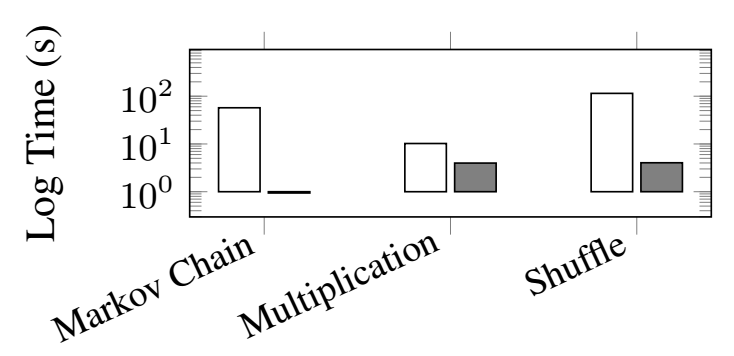
\includegraphics{results.png}
    \end{tikzfigure}

    Although \textbf{abstraction} for rich probabilistic models is a new and emerging
    field, recent work by Holtzen et al. \cite{DBLP:conf/icml/HoltzenBM18} shows
    \textbf{promising results} in applying \textbf{predicate abstraction} on
    probabilistic programs. \textbf{Our goal} is to consider a wide range of
    abstractions, understand their properties, and determine how to combine them
    in a successful manner.
  }

  \column{0.5}

  \block{Methodology}{
    \begin{tikzpicture}
      \node [object] (model) at (0, 0) {model};
      \node [object] (query) at (0, -3) {query};
      \node [process] (abstraction) at (6, -1.5) {abstraction};
      \node [object] (abstract_model) at (15, 1.5) {abstract model};
      \node [object] (abstract_query) at (15, -1.5) {abstract query};
      \node [object] (error_bound) at (15, -4.5) {error bound};
      \node [process] (inference2) at (23, 0) {inference};
      \node [object] (approximation) at (31, 0) {approximation};
      \node [process] (inference) at (0, -7.5) {inference};
      \node [object] (answer) at (31, -7.5) {answer};
      \node [process] (is_within) at (31, -4.5) {is within};

      \path [arrow,dashed] (model) -- (abstraction);
      \path [arrow,dashed] (query) -- (abstraction);
      \path [arrow,dashed] (abstraction) -- (abstract_model);
      \path [arrow,dashed] (abstraction) -- (abstract_query);
      \path [arrow,dashed] (abstraction) -- (error_bound);
      \path [arrow,dashed] (abstract_model) -- (inference2);
      \path [arrow,dashed] (abstract_query) -- (inference2);
      \path [arrow,dashed] (inference2) -- (approximation);
      \path [arrow] (model) -- (query) -- (inference);
      \path [arrow] (inference) -- (answer);
      \path [arrow,dashed] (approximation) -- (is_within);
      \path [arrow,dashed] (is_within) -- (answer);
      \path [arrow,dashed] (error_bound) -- (is_within);
    \end{tikzpicture}
    Abstraction can be used to improve inference speed by simplifying the model
    beforehand. We can find an abstract representation of a model
    specific to each query, and perform inference on the
    abstraction. The abstraction may be \textbf{exact} and produce the same
    answer as the original model, or it may produce a bounded approximation.
    An abstraction can be created by applying a combination of \textbf{atomic
    transformations} in a \textbf{greedy} manner.
  }

  \block{Impact}{
    This work is likely to result in significant improvements in
    \textbf{inference speed}, increase the \textbf{explainability} of models
    learned from data, and make the models more \textbf{scalable}.
  }

  \block{References}{
    \small
    \printbibliography[heading=none]
  }

\end{columns}
\end{document}